\section{Vorlesung 28.10.2016}
\subsection{Inzidenzstrukturen}
Struktur aus Punktmenge und Menge von Blöcken.\newline\newline
Tripel: (p,B,I)
\begin{itemize}
	\item p $\cap$ B = $\emptyset$
	\item I $\subseteq$ p x B
	\item p = Punkte - z.B. Vertices
	\item B = Blöcke - z.B. Kanten
	\item I = Inzidenzmatrix
\end{itemize}
Die Punkte p \glqq inzidieren\grqq{} demnach mit den Blöcken B, \glqq liegen auf\grqq{} einem Block. Dieser Block kann, wie in unserem Fall bei Graphen, eine Gerade sein.\newline

\subsubsection{Inzidenzmatrize - ungerichtete Graphen}
\begin{itemize}
	\item n Knoten, m Kanten
	\item n x m Marix B=b\textsubscript{i,j}
	\item G=(V,E)
\hspace*{3mm}V=\{v\textsubscript{1}, \ldots, v\textsubscript{n}\}\newline
\hspace*{3mm}E=\{e\textsubscript{1}, \ldots, e\textsubscript{m}\}\newline
\hspace*{3mm}$b\textsubscript{i,j}\begin{cases}1,\>v\textsubscript{i}\in e\textsubscript{j}\\0,\>sonst\end{cases}$\newline
\end{itemize}

\begin{tabular}{cccc}
 & a & b & c \\
1 & 1 & 0 & 0 \\
2 & 1 & 1 & 0 \\
3 & 0 & 1 & 0 \\
\end{tabular}
\newline\newline
In dieser Inzidenzmatrize steht Vertex 1 nur auf Kante a, Vertex 2 auf Kante a und b (kann nicht auf c liegen) und Vertex 3 auf Kante b. In Form einer Bildes könnte das so aussehen:\newline
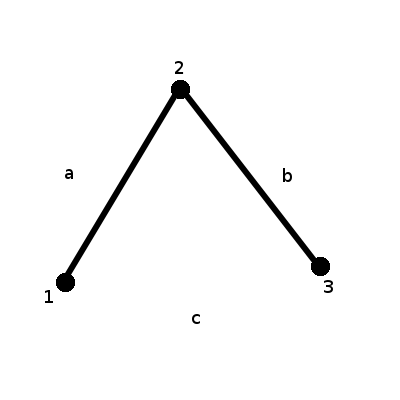
\includegraphics[width=0.4\textwidth]{lectures/161028/pix/dreieck.png}


\subsubsection{Inzidenzmatrize - gerichtete Graphen}
\begin{itemize}
	\item $b\textsubscript{i,j}\begin{cases}1,\>e\textsubscript{j}=(v\textsubscript{i},x)\\0,\>v\textsubscript{i}\ni e\textsubscript{j}\\-1,\>e\textsubscript{j}=(x,v\textsubscript{i})\end{cases}$\newline
\end{itemize}

\begin{tabular}{cccc}
 & a & b & c \\
1 & -1 & 0 & 0 \\
2 & 1 & 1 & 0 \\
3 & 0 & -1 & 0 \\
\end{tabular}\newline\newline
Hier sind die Kanten gerichtet. Im Gegensatz zur ungerichteten Inzidenzmatrize erhalten \glqq ankommende\grqq{} Kanten hier ein negatives Vorzeichen. Siehe Kante a zu Vertex 1 und Kante b zu Vertex 3.\newline
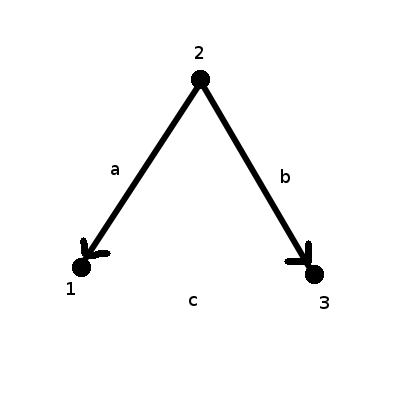
\includegraphics[width=0.4\textwidth]{lectures/161028/pix/dreieckge.png}

\newpage

\subsection{Laplace-Matrix}
\begin{itemize}
	\item G =(V,E)
	\item Gradmatrix D=d\textsubscript{i,j}
	\item Adjazenzmatrix A=a\textsubscript{i,j}
	\item Laplace-Mazrix \textit L = D-A = l\textsubscript{i,j}
\end{itemize}

$d\textsubscript{i,j}\begin{cases}deg(v\textsubscript{i}),\>i=j\\0,\>sonst\end{cases}$\newline\newline

$a\textsubscript{i,j}\begin{cases}1,\>(i,j)\in E\\0,\>sonst\end{cases}$\newline\newline
- A ist symmetrisch für ungerade Graphen\newline

$\textit{L}\begin{cases}deg(v\textsubscript{i}),\>i=j\\-1,\>i\neq j, (i,j) \in E \\0,\>sonst\end{cases}$\newline\newline
- Zusammenhang zur Inzidenzmatrix: \textit{L}=B x B\textsuperscript{T}\newline\newline

Beispiel:\\
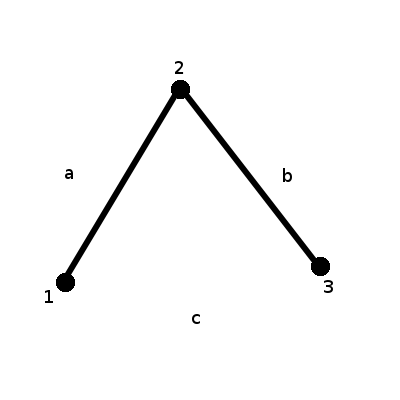
\includegraphics[width=0.4\textwidth]{lectures/161028/pix/dreieck.png}\\
Gradmatrix:\begin{tabular}{ccc}
1 & 0 & 0 \\
0 & 2 & 0 \\
0 & 0 & 1 \\
\end{tabular}
\\\\
Adjazenzmatrix:\begin{tabular}{ccc}
0 & 1 & 0 \\
1 & 0 & 1 \\
0 & 1 & 0 \\
\end{tabular}
\\\\
Laplace-Matrix:\begin{tabular}{ccc}
1 & -1 & 0 \\
-1 & 2 & -1 \\
0 & -1 & 1 \\
\end{tabular}

Eigenschaften:\\
\begin{itemize}
	\item symmetrisch
	\item die Zeilen- und Spaltensumme = 0
	\item Eigenwert $\lambda$\textsubscript{0}=0, v\textsubscript{0}=(1,\ldots,1) $\Rightarrow$ 2 v\textsubscript{0}=$\lambda$\textsubscript{0}
	\item Anzahl der 0 Eigenwerte $\Rightarrow$ Anzahl der connected components
	\item special gap: kleinster Eigenwert $\neq$ 0
	\item algebraische Konnektivität (Fiedler-Wert)
	\begin{itemize}
		\item zweit-kleinster Eigenwert - positiv-semidifinit
		\item $\lambda$\textsubscript{i} $\geq$ 0
	\end{itemize}
\end{itemize}

\subsubsection{Algebraische Konnektivität}
\begin{itemize}
	\item beschreibt wie gut verbunden der Graph, global gesehen, ist
	\item algebraische Konnektivität $\leq$ Vertex-Konnektivität
	\item $\mid$V$\mid$=n, min. Durchmesser von d(längster Pfad)
	\begin{itemize}
		\item alg. Konn $\geq$ 4/nd
	\end{itemize}
\end{itemize}

Beispiel:
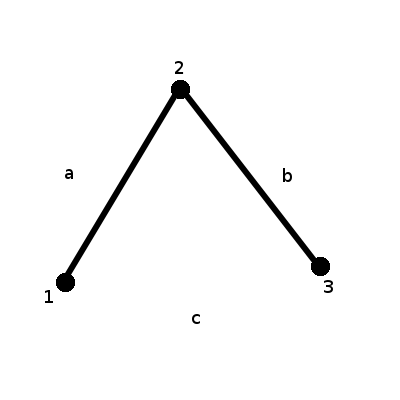
\includegraphics[width=0.4\textwidth]{lectures/161028/pix/dreieck.png}\newline
\begin{itemize}
	\item $\mid$V$\mid$=3
	\item d=2\newline
	\item vert. conn = 1
	\item alg. conn = $\lambda$\textsubscript{z} = 0,666 
\end{itemize}

\newpage

\subsubsection{Fiedler Vektor}
\begin{itemize}
	\item Eigenvektor zur Alg. Konn.
	\item eignet sich zur Graphpartitionierung
\end{itemize}

Beispiel:
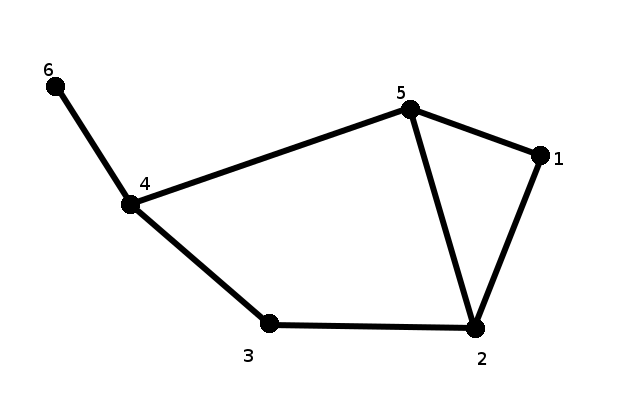
\includegraphics[width=0.4\textwidth]{lectures/161028/pix/fiedler.png}
\begin{itemize}
	\item F = $<$0.4, 0.3, 0.1, -0.2, 0.2, -0.8$>$
	\item \{4,6\},\{1,2,3,5\}\newline
\end{itemize}

\subsubsection{Interlacing Theorem}
\begin{itemize}
	\item Sei A eine reelle, symmetrische Matrix
	\item mit Eigenvektoren $\lambda$\textsubscript{1}$\geq$$\lambda$\textsubscript{2}$\geq$\ldots$\geq$$\lambda$\textsubscript{n}
	\item sei A\grq{} principal Submatrix von A
	\item Beispiel: principal Submatrix $\Leftrightarrow$ induzierter Subgraph, ein Vertex weniger (G-\{v\textsubscript{i}\})
	\begin{itemize}
		\item Eigenwerte zu A\grq{}: $\eta$\textsubscript{1} $\geq$ $\eta$\textsubscript{2} $\geq$ \ldots $\geq$ $\eta$\textsubscript{n-1}
		\item dann gilt: $\lambda$\textsubscript{i} $\geq$ $\eta$\textsubscript{i} $\geq$ $\lambda$\textsubscript{i+1} ... i = 1, 2,\ldots, n-1
	\end{itemize}
\end{itemize}

\subsubsection{Anzahl nicht-isomorpher Graphen}
\begin{itemize}
	\item V = \{1,\ldots,n\}
	\item E $\subseteq$ $\left(\begin{array}{c} V \\ 2 \end{array}\right)$ = [v]\textsuperscript{2}
	\item wie viele versch. Graphen gibt es?\\ $\Rightarrow$ $2^{\binom{n}{2}}$
	\begin{itemize}
		\item einige dieser Graphen sind isomorph zueinander
		\item wie viele Äquivalenzklassen gibt es für ($\cong$) auf V = \{1,-, n\}?
	\end{itemize}
\end{itemize}

\textbf{Approximation:}\newline
\begin{itemize}
	\item wie viele isomorphe Graphen gibt es für 6?
	\item Isomorpge-Bijektion $\pi$ V$\rightarrow$V
	\item Anzahl Permutationen: n!
	\item Es gib maximal n! isomorphe Graphen auf G\\
	
\hspace*{2cm}$\frac{2^\frac{n}{2}}{n!}=\frac{\text{Anzahl Graphen}}{\text{mgl. Bijektion fur einen einzelnen Graphen}}$\\
	\item wir haben mit $\frac{2^\frac{n}{2}}{n!}$ paarweise nicht-isomorphe Graphen\\
\hspace*{2cm}n!$\leq$n\textsuperscript{n}\newline
\hspace*{2cm}$log_2(2^{\begin{pmatrix}n\\2\end{pmatrix}}) = \begin{pmatrix}n\\2\end{pmatrix} = \frac{n^2}{2}(1-\frac{1}{n})$\newline
$log_2(\frac{2^{\begin{pmatrix}n\\2\end{pmatrix}}}{n!}) = \begin{pmatrix}n\\2\end{pmatrix} - log(n!) \geq \frac{1}{2}n^2-\frac{1}{2}n-n log_2(n)$\newline
\hspace*{5.2cm}$=\frac{n^2}{2}(1-\frac{1}{n}-\frac{2 log_2(n)}{n})$\newline
Fehler geht gegen $0 (2^{O(n^2)})$
\end{itemize}

\subsubsection{Isomorphismus auf Bäumen}
\begin{itemize}
	\item das \glqq das ist einfach\grqq{} $\rightarrow$ Programm mit polynomieller Zeit bauen
	\item Baum codieren via 2n 0en und 1en\\
\hspace*{2cm}$\hookrightarrow$ das sei der Code von Baum T
	\item zu beweisen: isomorph Bäume haben gleiche codes
	\item drei Klassen von Bäumen:
	\begin{itemize}
		\item Bäume
		\item gewurzelte Bäume
		\item gewurzelte Bäume mit Geschwisterordnung
	\end{itemize}
\end{itemize}
\newpage

Beispiel:\\
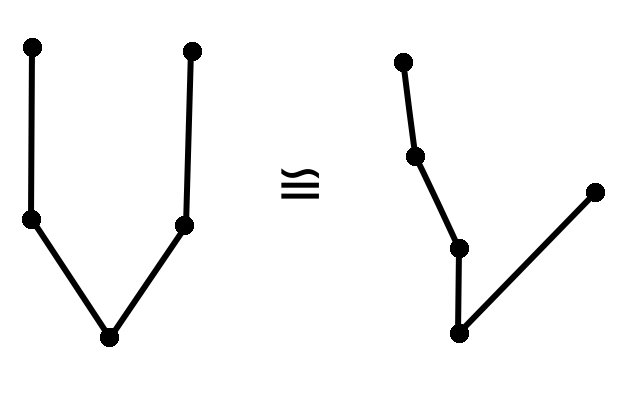
\includegraphics[width=0.4\textwidth]{lectures/161028/pix/graph1.png}
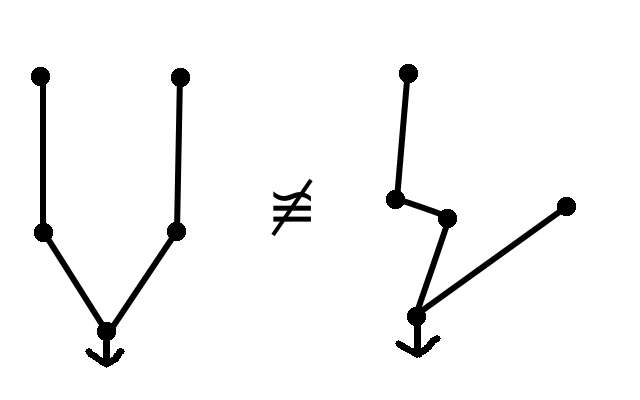
\includegraphics[width=0.4\textwidth]{lectures/161028/pix/graph2.png}\\
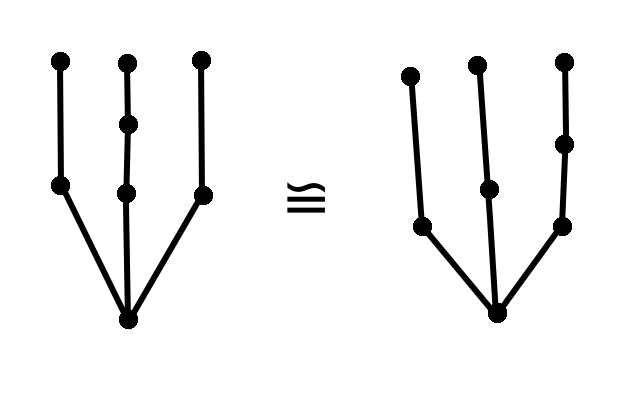
\includegraphics[width=0.4\textwidth]{lectures/161028/pix/graph3.png}\\

\textbf{Algorithmus (gewurzelt, geordnet):}\newline
\begin{itemize}
	\item K1: Blätter werden kodiert als 01
	\item K2: v $\in$ V mit Kiner c\textsubscript{1},\ldots,c\textsubscript{n} $\in$ V
	\item Sei A\textsubscript{i} der Code von c\textsubscript{i}
	\item Dann codiert 0 A\textsubscript{1}\_A\textsubscript{n} 1
	\begin{itemize}
		\item Isomorphe Bäume werden mit gleichem Code codiert
		\item Baum aus Code: Zeigt das nicht-isomorphe Bäume verschiedenen Code haben
	\end{itemize}
\end{itemize}
Beispiel:\\
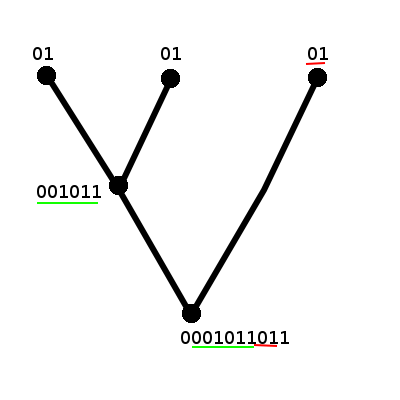
\includegraphics[width=0.4\textwidth]{lectures/161028/pix/isomorph.png}
\newpage

\textbf{Induktion:}\newline
\begin{itemize}
	\item einzelne Wurzel \glq 01\grqq{}
	\item Schritt: Code K, Länge 2(n+1) mit Form 0A1, A=A\textsubscript{1}\_\textsubscript{n}\\
bestimme A\textsubscript{1}: Kleinster 0/1 kann mit gleicher Zahl von 0 und 1\newline
	\item A\textsubscript{i} ist via Induktion des Codes für dazugehörigen gewurzelten, geordneten Baum T\textsubscript{i}
\end{itemize}

\glq Kleinste maximale Entfernung zwischen den Blättern als Wurzel wählen \grqq{}